\chapter{Why?}
\label{chapter:Introduction}
\graphicspath{ {./chapter00/Fig} }


Welcome to Introduction to Digital Design - A Datapath and Control Approach.  
You might be tempted to ask ``Why bother writing yet another digital design 
text?''  The assumption being that this text is going to cover the same ground as a 
typical digital design text.  And yes, to some  degree it will, but more importantly 
it will not.   \emph{This text presents a systematic approach to the design process for 
digital circuits that will enable you to design sophisticated digital systems.} I consider a
digital design sophisticated when it needs to be described algorithmically.

After going through this text and laboratories my goal is that you should be able to
use 100\% of the material you learned to design a digital systems that in 
Figure~\ref{fig:introAbstract}.

\begin{figure}[ht]
\center{\scalebox{0.7}{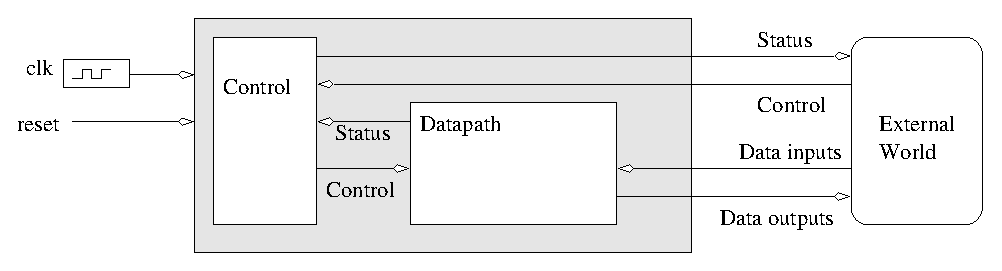
\includegraphics{../../chapter08/Fig/Abstract}}}
\caption{An abstract digital system constructed from a datapath and a control unit.}
\label{fig:introAbstract}
\end{figure}

The datapath and control framework classifies the inputs and outputs of every
digital logic building block as either \textbf{Data inputs}, \textbf{Data output}, \textbf{Control inputs}, 
\textbf{Status output} (the two special signals, \textbf{clk} and \textbf{reset} sit outside this
classification).  Under this framework, the datapath performs all data manipulations and the 
control unit sequences the control inputs for datapath.  The datapath is built from
combinational and sequential building blocks like multiplexers and counters.  The control unit
is a finite state machine.

\subsection{Class Organization}
 I wrote the text, homework and laboratory 
exercises for a 4-credit course delivery.  The example timeline shown in Table~\ref{table:introTimeline} assumes
3 50-minute lectures per week and 1 2/3-hour laboratory a week. 

\subsection{Laboratory}
While it is expected that students finish the laboratory
during the scheduled time, frequently students will need additional time to complete work, so accommodations need
to be in-place for them to access the hardware and software outside of course hours.   I expect that my students will 
need to work about 4-hours a week outside of class. 



\section{Example Timeline}

\begin{longtable}{|l|m{7cm}|l|l|}
\caption{The labs in this example timeline are shown the earliest possible
to insure that the prerequisite skills have been covered or 3 lecture sessions
have passed since the last lecture.}
\label{table:introTimeline}\tabularnewline
\toprule()
Session  & Topic & Assignment & Reading \\
\bottomrule()
\endfirsthead
\toprule()
Session  & Topic & Assignment & Reading \\
\endhead
1			&  Course Intro, Binary numbering, Hexadecimal & & 1.1 -- 1.3 \\ \hline
2			& Binary Addition & & 1.4 \\ \hline
3			& Logic gates / Circuit to Symbolic / Circuit to Truth Table & & 2.1, 2.21, 2.2.2 \\ \hline
4			& Symbolic to Truth Table / Symbolic to Circuit & HW\#1 Due & 2.2.3, 2.2.4 \\ \hline
5 			& Symbolic to Verilog & & Supplemental \\ \hline
 \rowcolor{yellow} 
Lab \#1	& Introduction to CAD tools and Verilog & & \\ \hline
6 			& Symbolic to Symbolic & & 2.2.5 \\ \hline
7 			& Symbolic to Symbolic & & 2.2.5 \\ \hline
8 			& Truth Table to Symbolic SOP and POS & HW\#2 Due & 2.2.6, 2.2.7, 2.3 \\ \hline
 \rowcolor{yellow} 
Lab \#2 	& Hexadecimal to 7-segment Converter & Lab \#1 Due & \\ \hline
9 			& Karnaugh Maps, 3 variables & & 3.1 \\ \hline
10			&  Combinational Logic with Verilog & & Supplemental \\ \hline
11 			& Karnaugh Maps, 4 and 5 variables & HW\#3 Due & 3.2, 3.3 \\ \hline
 \rowcolor{yellow} 
Lab \#3	& Rock Paper Scissors & Lab \#2 Due & \\ \hline
12 			& Don't cares & & 3.5 \\ \hline
13			& SOP and POS in Karnaugh maps & & \\ \hline
14 			& Exam Review & HW\#4 Due & 3.6 \\ \hline
 \rowcolor{yellow} 
Lab \#4 	& Guessing Game & Lab \#3 Due & \\ \hline
15			& Exam I & & \\ \hline
16 			& Decoder / Multiplexers & & 4.1, 4.2 \\ \hline
17 			& 2's complement & & 1.5 \\ \hline
18 			& Adders & HW\#5 Due & 4.3 \\ \hline
19			& Adder Subtractor & & 4.4 \\ \hline
 \rowcolor{yellow} 
Lab \#5 	& Guessing Game with Hints & Lab \#4 Due & \\ \hline
20			& Comparator & & 4.5 \\ \hline
21			& Wire Logic / Combinations & & 4.7, 4.8 \\ \hline
22			& SR Latch & HW\#6 Due & 5.5 \\ \hline
23			& Basic memory elements -- timing & & 5.1 \\ \hline
24			& Basic memory elements -- practical considerations & & 5.7 \\ \hline
 \rowcolor{yellow} 
Lab \#6 	& Decimal Calculator & Lab \#5 Due & \\ \hline
25 			& Register & HW\#7 Due & 6.1 \\ \hline
26 			& Shift Registers & & 6.2 \\ \hline
27 			& Counter & & 6.3 \\ \hline
 \rowcolor{yellow} 
Lab \#7 	& 1 Dimensional Cellular Automata & Lab \#6 Due & 6.3 \\ \hline
28 			& RAM & & 6.4 \\ \hline
29 			& Register Transfer & & 6.5 \\ \hline
30			& Exam Review & HW\#8 Due & Supplemental \\ \hline
 \rowcolor{yellow} 
Lab \#8 	& Mod 10 Counter & Lab \#7 Due & \\ \hline
31			& Exam II & & \\ \hline
32 			& Sequential Design -- Traffic Light Controller & & 7.4 \\ \hline
33 			& Sequential Design -- Verilog & & Supplemental \\ \hline
 \rowcolor{yellow} 
Lab \#9 	& Stopwatch Datapath & Lab \#8 Due & \\ \hline
34 			& Sequential Design -- Timing & & 7.6 \\			 \hline
35 			& Sequential Design -- Vending Machine & HW\#9 Due & 7.5 \\ \hline
 \rowcolor{yellow} 
Lab\#10 	& Stopwatch Control & Lab \#9 Due & \\ \hline
36 			& Datapath and Control Theory & & 8.1, 8.2, 8.3 \\ \hline
37 			& Datapath and Control Theory & & 8.1, 8.2, 8.3 \\ \hline
38 			& Datapath and Control Practice & HW\#10 Due & 8.4, 8.5 \\ \hline
 \rowcolor{yellow} 
Lab\#11	& Stopwatch -- Datapath and Control & Lab \#10 & \\ \hline
39			& Datapath and Control Practice & & 8.4, 8.5 \\ \hline
40			& Datapath and Control Timing & & 8.4, 8.5 \\ \hline
41			& Datapath and Control Practice & & 8.7 \\ \hline
 \rowcolor{yellow} 
			& Lab wrap-up & Lab \#11 Due & \\ \hline
42			& Exam Review & HW\#11 Due & Supplemental \\ \hline
			& Exam III & & \\ \hline
\end{longtable}